\section{Molekulare Stoffe}
Moleküle sind abgeschlossene Atomverbände aus nichtmetallischen Atomen. 

\subsection{Bildung von Molekülen aus Atomen}
Atombindung (kovalente Bindung): Gemeinsames bindendes Elektronenpaar zwischen 2 Nichtmetallatomen. 

\subsubsection{Lewisformel}
\begin{multicols}{2}
$F_2$: \ \chemfig{\Lewis{0.246,F}+\Lewis{024.6, F}}  $\Rightarrow$  \chemfig{\Lewis{246,F}-\Lewis{026,F}} \\
$O_2$: \ \chemfig{\Lewis{0.246., O}+\Lewis{024.6., O}} $\Rightarrow$ \chemfig{\Lewis{35, O}=\Lewis{17, O}} \\
$N_2$: \ \chemfig{\Lewis{0.2.46., N}+\Lewis{02.4.6., N}} $\Rightarrow$ \chemfig{\Lewis{4, N}~\Lewis{0, N}} \\
$C_2Cl_2$: \ \chemfig{\Lewis{246, Cl}-[,0.7]C~[,0.7]C-[,0.7]\Lewis{026, Cl}}
\end{multicols}

\subsubsection{EPA-Modell}
Elektronenpaare stossen sich gegenseitig maximal ab. Damit kann die räumliche Struktur vorausgesagt werden. Bei vier Valenz-Kugelwolken beträgt der Winkel dazwischen $109.5^\degree$ (Tetraederwinkel).

\subsection{Elektronegativität (EN)}
Fähigkeit eines Atoms, Bindungselektronen anzuziehen. Die EN ist grösser, je grösser die Rumpfladung und je kleiner der Rumpfradius ist. $EN=\frac{Rumpfladung}{Rumpfgroesse}$

\subsection{Polare Bindung}
Polarität einer Bindung: $\Delta EN = | EN_{1} - EN_{2} |$. 
\begin{itemize}
	\item $\Delta EN = 0$: apolare Bindung
	\item $\Delta EN = 0 .. 1.5$: polare Bindung
	\item $\Delta EN > 1.5$: ionische Bindung
\end{itemize}

Moleküle sind Dipole (polare Moleküle), wenn die Schwerpunkte der Partialladungen nicht zusammenfallen.

\chemfig{\underset{3.0}{Cl}-\underset{3.0}{Cl}} $\Rightarrow \Delta EN=0$ apolare Bindung \\
\chemfig{\overset{\delta+}{\underset{2.1}{H}}-\overset{\delta-}{\underset{3.0}{Cl}}} $\Rightarrow \Delta EN=0.9$ polare Bindung \\
\chemfig{\underset{0.9}{Na^+}-\underset{3.0}{Cl^-}} $\Rightarrow \Delta EN=2.1$ ionische Bindung 

\subsection{Zwischenmolekulare Kräfte}
Anziehende Kräfte, die zwischen Molekülen herrschen und Stoffeigenschaften (mp,bp; Mischbarkeit; Viskosität; Oberflächenspannung; ...) beeinflussen. Normalerweise schwächer als kovalente Bindungen.

\begin{itemize}
	\item Dipol-Dipol Kräfte: gegenseitige Anziehung von Dipolmolekülen aufgrund unterschiedlicher Partialladungen. Je polarer, desto grösser.
	\item Van-der-Waals Kräfte: gegenseitige Anziehung von unpolaren Molekülen aufgrund kurzzeitig ungleichmässig verteilter Elektronen. Sehr schwach, mehr $e^-$ $\Rightarrow$ stärker, zwischen allen Molekülen
	\item Wasserstoffbrücken (H-Brücken): Anziehung zwischen stark positiv polarisierten H-Atomen und freien Elektronenpaaren von stark elektronegativen Atomen (F,O,N) $\Rightarrow$ existieren nur bei H-F, H-O oder H-N Bindungen. Stärkste zwischenmolekulare Kräfte.
\end{itemize}

\subsubsection{Siedepunkt abschätzen}
Prinzip: Beim Verdampfen müssen zwischenmolekulare Kräfte überwunden werden $\Rightarrow$ grosse zw.molek. Kräfte $\Leftrightarrow$ hoher Siedepunkt. 

\textbf{Beispiel:} Wasser bildet alle zwischenmolekularen Kräfte aus, das erklärt den höchsten Siedepunkt. $H_2Te$ bildet ausschliesslich VdW-Kräfte aus, weshalb der Siedepunkt eher tief ist.
\begin{figure}[htbp]
	\centering
	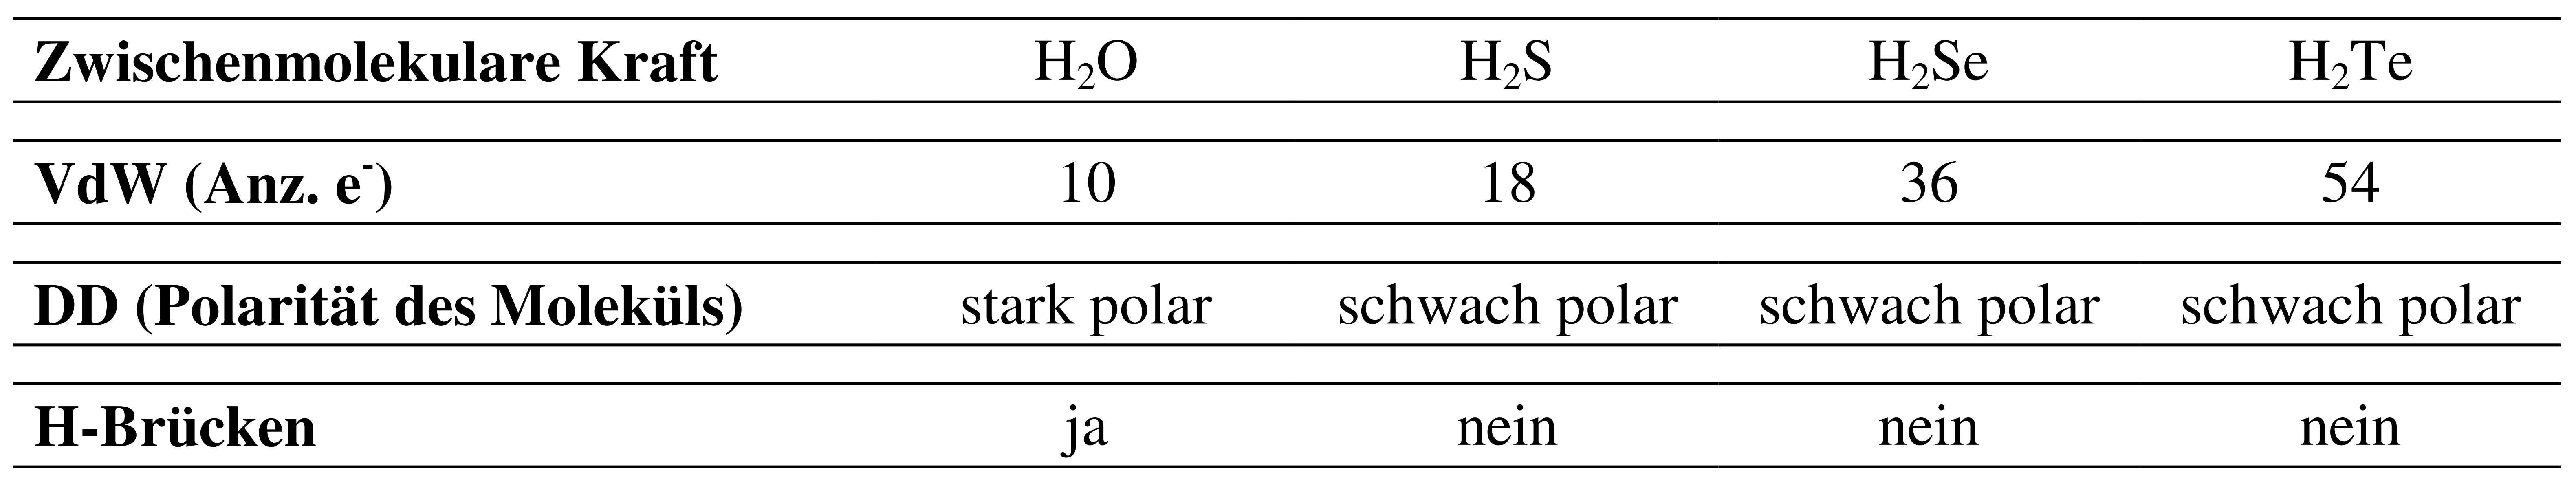
\includegraphics[width=1\linewidth]{images/5_Siedepunkt.png}
\end{figure}

\subsubsection{Löslichkeit abschätzen}
Prinzip: Ein molekularer Stoff ist löslich, wenn er mit dem Lösungsmittel dieselbe Art zwischenmolekularer Kräfte ausbilden kann. \\
Halbpolare Stoffe besitzen eine polare Gruppe (z.B. -OH) und einen nicht zu langen unpolaren Teil (z.B. KW-Kette). Je länger die KW-Kette desto hydrophober, schlechter löslich wird das Molekül.

\subsubsection{Zersetzung}
Bestimmte molekular aufgebaute Stoffe haben keinen Siedepunkt. Werden solche Stoffe erwärmt, zersetzen sie sich, d.h. Atombindungen im Molekül werden gebrochen und die Atome verknüpfen sich neu.

\subsection{Flüssigkristalle}
\subsubsection{Aggregatszustände}
\begin{itemize}
	\item fest: Moleküle mit 3-dimensionale Fernordnung, anisotrop (richtungsabhängig)
	\item flüssig: ungeordnete Moleküle, isotrop
	\item flüssigkristallin: Moleküle mit 1- oder 2-dimensionaler Fernordnung
\end{itemize}

\subsubsection{Phasen der Flüssigkristalle}
\begin{figure}[htbp]
	\centering
	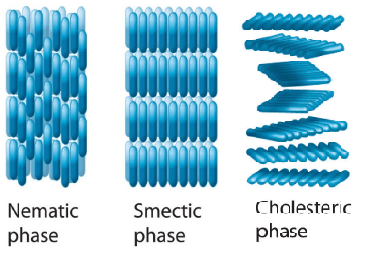
\includegraphics[width=0.5\linewidth]{images/11_Phasen.png}
\end{figure}
\begin{itemize}
	\item nemantische Phase
		\begin{itemize}
			\item 1-dimensionale Ordnung
			\item Moleküle entlang Längsachse ausgerichtet
			\item Molekülenden nicht geordnet
			\item Aneinander Vorbeigleiten möglich
		\end{itemize}
	\item smektische Phase
		\begin{itemize}
			\item 2-dimensionale Ordnung
			\item Moleküle entlang Längsachse ausgerichtet
			\item Molekülenden geordnet $\Rightarrow$ Entstehung von Schichten
			\item Aneinander Vorbeigleiten nicht möglich
			\item SmA: Längsachse in $90^\circ$-Winkel zur Schicht
			\item SmC: Längsachse geneigt zur Schicht
		\end{itemize}
	\item cholestrische Phase
		\begin{itemize}
			\item Schichten mit nematischer Ordnung
			\item jede Schicht um charakteristischen Winkel verdreht (Abstossungskräfte)
			\item Schraubenförmige (helikale) Struktur mit Periodizität im nm-Bereich.
		\end{itemize}
\end{itemize}

\subsubsection{Atomarer Aufbau}
Flüssigkristalle bestehen aus langen, stabartigen Molekülen mit starren Atomgruppen. 

\begin{figure}[htbp]
	\centering
	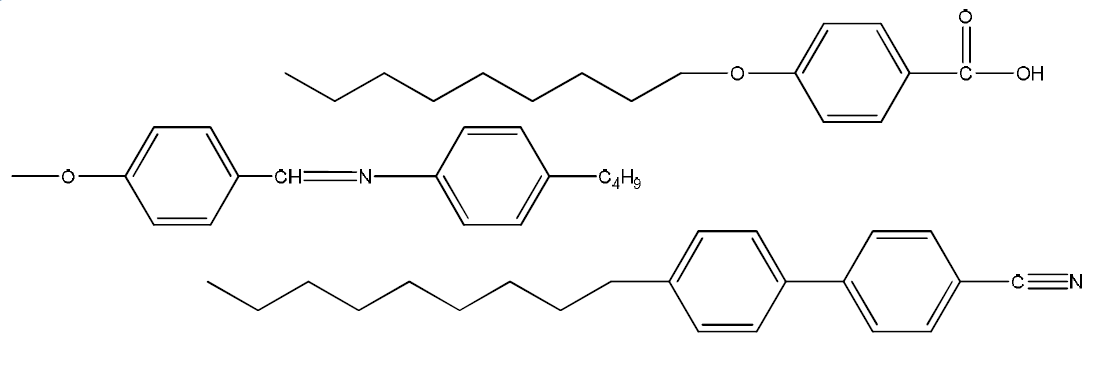
\includegraphics[width=0.8\linewidth]{images/11_Atome.png}
\end{figure}

Zwischenmolekulare Kräfte schränken die Beweglichkeit ein, die Stäbchen richten sich deshalb parallel aus. Da die Atomgruppen meist polar sind, entstehen Dipol-Dipol Kräfte und extern angelegte elektrische Felder können die Moleküle ausrichten (Prinzip des LCD Displays). 